\chapter{Non-monotonic Reasoning}
\label{chapter:defeasible-reasoning}

The study of logical systems that violate the property of monotonicity has received significant attention over the
past few decades. The motivation for such systems arises from the observation that, in many contexts, it is useful
to adopt a more credulous stance on inference—one that allows conclusions to be drawn even when knowledge is
incomplete or uncertain. In everyday reasoning, it is often necessary to reach conclusions despite imperfect
information about the world.

Within the confines of monotonicity, once an inference has been made, no amount of new information would result in
its subsequent retraction. This restriction ensures that inferences are only drawn when they are absolutely
certain. Such a restriction may be undesirable: if one were permitted to withdraw conclusions upon learning new,
relevant, and possibly contradictory information, reasoning could become more flexible---allowing beliefs to
evolve as knowledge changes.

While the range of non-monotonic systems is fairly broad, this work is only interested in one particular style of
reasoning developed by Kraus, Lehmann, and Magidor \shortcite{kraus1990nonmonotonic,lehmann1992what}. This system
is usually referred to by the initialisation of the authors, and so we speak about the \textit{KLM framework for
	defeasible reasoning}.

\section{Background on Non-monotonic Reasoning}
\label{section:nmr-background}

Near the end of the previous chapter, the matter of consequence was discussed in a very formal sense. In order to
make explicit the ways in which monotonic inference systems are undesirable, it will be useful to first
distinguish precisely this formal treatment from the colloquial understanding of consequence, as reasoning done
with the formal approach may display certain un-intuitive results
\cite{tarski1936consequence,kraus1990nonmonotonic}. As a demonstration of such a result, we consider the following
knowledge base, consisting of propositions conveying the information that \textit{humans experience
	chronological-time} and that \textit{soldiers are human}.

\begin{center}
	\begin{varwidth}{\textwidth}
		\begin{enumerate}[nosep]
			\item $\texttt{human} \rightarrow \texttt{chronological-time}$ \label[proposition]{prop:1}
			\item $\texttt{soldier}\rightarrow \texttt{human}$ \label[proposition]{prop:2}
			\item $\texttt{Billy Pilgrim}\rightarrow \neg \texttt{chronological-time}$ \label[proposition]{prop:3}
		\end{enumerate}
	\end{varwidth}
\end{center}

With these propositions in mind, suppose one were to encounter a solider. It would be sensible to deduce, by
\Cref{prop:4,prop:2,prop:1}, that the encountered individual experienced chronological time. Suppose that after a
short period of time, the soldier introduced themself as \textit{Billy Pilgrim}. One reasonable course of action
might be to incorporate the new information, that \textit{Billy Pilgrim is a soldier} into our knowledge base, as
the rule:

\begin{center}
	\begin{varwidth}{\textwidth}
		\begin{enumerate}[nosep]
			\setcounter{enumi}{3}
			\item $\texttt{Billy Pilgrim} \rightarrow \texttt{soldier}$ \label[proposition]{prop:4}
		\end{enumerate}
	\end{varwidth}
\end{center}

The addition of this rule seems results in some tension between two deductions. On the one hand, it was previously
deduced that the individual experienced time chronologically; now it seems reasonable to deduce that they
experience time non-chronologically. A pragmatic reasoning would likely recognise that while the initial deduction
was reasonable at the time, the subsequent learning of more specific information should result it's retraction, to
be replaced by a new deduction made from a more informed epistemic position. Such recourse is not available to
classical logics: by the principle of explosion, if our theory entails \texttt{chronological-time} and $\neg
	\texttt{chronological-time}$, then it is is inconsistent. Any inconsistency renders the theory trivial, as an
inconsistent theory entails everything—and therefore conveys nothing meaningful.

Examining the same situation from a semantic perspective, it is clear that is not as bad as was originally feared:
indeed the knowledge base containing \Crefrange{prop:1}{prop:4} is satisfiable; specifically it has the following
four models:
\begin{center}
	\begin{varwidth}{\textwidth}
		\begin{enumerate}[nosep]
			\item $\{\overline{{b}},\overline{{h}},\overline{{c}},\overline{{s}}\}$
			\item $\{\overline{{b}},\overline{{h}},{c},\overline{{s}}\}$
			\item $\{\overline{{b}},{h},{c},\overline{{s}}\}$
			\item $\{\overline{{b}},{{h}},{{c}},{{s}}\}$
		\end{enumerate}
	\end{varwidth}
\end{center}
%
For clarity, $b,c,h,s$ represent the propositional atoms \texttt{Billy Pilgrim, chronological time, human,} and
\texttt{soldier}, respectively. One notable observation is that, in each of these models, $\texttt{Billy Pilgrim}$
is assigned the value \texttt{false}. Consequently, the knowledge base entails $\neg \texttt{Billy Pilgrim}$. If
the belief that the soldier introduced themself truthfully---requiring that the knowledge base contain the
additonal fact that \texttt{Billy Pilgrim} is \texttt{true}---then the theory is inconsistent. Perhaps it would be
more advisable to doubt the veracity of the soldier's introduction, and in doing so maintain a consistent theory.
That is, Billy Pilgrim remains a solider, just not the one that was encountered. However, if this position is
adopted, the effects are much more severe than not believing the solider: one must accept that no truthful
introduction to Billy Pilgrim can ever occur, as his existence is rendered impossible.

This property---that adding new information can never result in retraction of prior knowledge---is called
monotonicity. The presence of monotonicity prevents one from making inferences that we are not absolutely certain
of. Intuitively, this means we may not infer anything that does not hold in all the possible worlds, relative to
what we already know. In other words, only infer that which is true in every model of our current knowledge. If we
remain in the classical realm, it seems our only options are to abandon our original claim or risk explosion.

At this point it is a good idea to provide some early intuitions on how one might violate monotonicity in a
reasonable way. Continuing with the example, it is reasonable to suggest that typically we think think that humans
expereince time chronologically. In order to reconcile the information that Billy Pilgrim is a human who
experiences non-chronological time, it could be that he is simply an a-typical human. In the proceeding section,
these ideas will be explored in a more formal manner. The idea observed by Shoham
\shortcite{shohamSemanticApproach}, that we may ``bend the rules'' of logical consequence and restrict
consideration to privileged subsets of valuations deemed `preferable' is foundational to this kind of reasoning.

\section{Preferential Reasoning and the KLM Framework}
\label{section:klm-framework}

The KLM framework for non-monotonic reasoning was initially described by a collection of consequence relations
satisfying certain axioms, frequently called the \textit{rationality postulates}. These axioms describe a
reasonable account of non-monotonic consequence. We borrow a nice story from Dov Gabbay
\shortcite{gabbay1985theoreticalFoundations}, in which he motivates why consequence relations are a good starting
point for the study of non-monotonic systems.

Paraphrasing, the reader to imagine a machine that is supposed to do some kind of non-monotonic inference. The
machine maps meaningful expressions of knowledge onto formulae, and so queries of the form \say{Does $\phi$ follow
	(non-monotonically) from $\psi$?}. Something goes awry (suppose some coffee was spilled), calling into question
whether the logic of the machine still functions correctly. Even worse, the interface, which provides the mapping
between formulae and which concrete pieces of knowledge they represent, is destroyed. Consequently, if the machine
functions correctly cannot be determined based on its output since the meaning represented by each formula cannot
be ascertained. How might one then evaluate the machine's function? If we were interested in classical
consequence, we would be well-equipped to assess the correctness of the machine by determining if it satisfied
reflexivity, monotonicity, and cut (we point to \Cref{definition:consequence-relations} as a reminder). In other
words, to study the more abstract properties of consequence.

This is precisely the starting point that Kraus, Lehmann, and Magidor took up \shortcite{kraus1990nonmonotonic},
suggesting that before getting to the semantics of a non-monotonic system, it is a good idea to axiomatise the
system as a consequence relation satisfying certain properties. The rationality postulates are precisely this
axiomatisation, characterising a sensible pattern of reasoning for non-monotonic systems. The symbol `$\twiddle$'
(pronounced ``twiddle'') is used instead of `$\vdash$' to denote a non-monotonic consequence relation. As may be
expected, $\phi \twiddle \psi$ has the same meaning as $(\phi, \psi) \in \; \twiddle$, and $\phi \ntwiddle \psi$
as $(\phi, \psi)\not \in \; \twiddle$. At times of potential confusion, a subscript may be used to disambiguate
which consequence relation is being referred to, and so $\twiddle_{p}$ would refer to a preferential relation, as
defined below.

\subsection{Preferential Consequence Relations}
\label{subsection:system-P} \index{non-monotonic reasoning! preferential}

We begin the exposition of the KLM framework by looking at \textit{preferential consequence}, or \textit{system
	P}.

\begin{definition}
	\label{definition:preferential-relation} \index{preferential!consequence relations}

	The consequence relation $\twiddle$ is a \emph{preferential consequence relation} if and only if it satisfies the
	properties of \emph{Reflexivity}, \emph{Left Logical Equivalence}, \emph{Right Weakening}, \emph{And}, \emph{Or},
	and \emph{Cautious Monotony}.
\end{definition}
%
Each property, or postulate, of preferential relations is presented in a style analogous to inference rules. The
intended meaning is that, if all statements above the line are included in the relation, then the statement below
must also be included.
%
\begin{align}
	\label[postulate]{postulate:ref}
	\inferLeft{Reflexivity}{}{\phi \twiddle \phi}
\end{align}
%
The first axiom, \textit{Reflexivity}, is largely self justifying. It makes little sense to speak about a notion
of consequence that does not satisfy this property. Such systems are discussed in
\Cref{subsection:association-rules}, although we are reluctant to call them ``logical''.
%
\begin{align}
	\label[postulate]{postulate:lle}
	\inferLeft{Left Logical Equivalence}{\vdash \phi \leftrightarrow \psi, \quad \phi \twiddle \gamma}{\psi \twiddle \gamma}
\end{align}
%
The justification for \textit{Left Logical Equivalence} is a bit more opaque. The principle it describes is that
if two scenarios represent the same state of affairs, and in one of these scenarios it we typically expect some
consequence, then we should expect the same in the other scenario. \textcolor{red}{Invariant to substitution of
	logically equivalent formulas? Yes! So, syntax-independent}
%
\begin{align}
	\label[postulate]{postulate:rw}
	\inferLeft{Right Weakning}{\vdash \psi \rightarrow \gamma, \quad \phi \twiddle \psi}{\phi \twiddle \gamma}
\end{align}
%
\textit{Right Weakening} allows the preservation of classical consequence within preferential logic. It says that,
if from $\phi$ we normally expect $\psi$, but from $\psi$ we \textit{always} see $\gamma$, then we are entitled to
think that from $\phi$ we normally expect $\gamma$ as well.
%
\begin{align}
	\label[postulate]{postulate:or}
	\inferLeft{Or}{\phi \twiddle \gamma, \quad \psi \twiddle \gamma}{\phi \lor \psi \twiddle \gamma}
\end{align}
%
As a justification for \textit{Or}, consider that \textit{Normally, if Billy were abducted by aliens he would be
	traumatised}, but also \textit{Normally, if Billy witnessed the fire-bombing of Dresden he would be traumatised}.
If we learned that either of these events took place, we should find it plausible to infer that Billy were
traumatised.
%
\begin{align}
	\label[postulate]{postulate:and}
	\inferLeft{And}{\phi \twiddle \psi, \quad \phi \twiddle \gamma}{\phi \twiddle \psi \land \gamma}
\end{align}
The \textit{And} postulate suggests that if $\psi$ and $\gamma$ are both expected consequence of $\phi$, then
their conjunction is also expected. This postulate fails in probabilistic systems, such as \textit{association
	rules} \cite{gabbay1985theoreticalFoundations}.
\begin{align}
	\label[postulate]{postulate:cm}
	\inferLeft{Cautious Monotony}{\phi \twiddle \psi, \quad \phi \twiddle \gamma }{\phi \land \psi \twiddle \gamma}
\end{align}
\textit{Cautious Monotony} (which has also be called \textit{Cumulative Monotony} by \cite{makinson2003bridges},
and \textit{Restricted Monotony} by \cite{gabbay1985theoreticalFoundations}) corresponds to the notion that if we
are in an epistemic state $\phi$ where one expectation, among others, is that $\psi$ holds. Learning that $\psi$
indeed holds should not alter the epistemic state in such a way that the \textit{other} expectations are
abandoned, and so the new state, $\phi \land \psi$, we should expect everything that was expected when all we knew
was $\phi$. In other words, we reason monotonically with respect to expected information. The above postulates
capture the essence of preferential (consequence) relations. Much like we saw with Hilbert systems, however,
certain rules, which reveal interesting properties of system P, may be derived. A version of \textit{Cut}:
\begin{align}
	\label{postulate:cut}
	\inferLeft{Cut}{\phi \land \psi \twiddle \gamma, \quad \phi \twiddle \psi}{\phi \twiddle \gamma}
\end{align}
The original version due to Gentzen \cite{Ben1993Mathematical}, which is presented as:
\begin{align}
	\inferLeft{Monotonic Cut}{\phi \land \psi \twiddle \gamma, \quad \alpha \twiddle \psi}{\phi \land \alpha \twiddle \gamma}.
\end{align}
This construction implies monotonicity as it requires that the typical consequence of $\alpha$, which is $\psi$,
must remain a consequence when the conjunction $\alpha \land \phi$ is considered. The former variation does not
enforce this, and rather says \say{Suppose I have certain knowledge of $\phi$, and that if I were to assume $\psi$
	I should expect to conclude $\gamma$. Then if I can show that infact $\psi$ was already an expected consequence of
	knowing $\phi$, I should expect that $\gamma$ follows from $\phi$ }. When considered alongside the argument for
Cautious Monotony, Cut seems acceptable.

The rule $S$, which is analogous to one half of the deduction theorem (cf. \Cref{axiom:deduction-theorem}),
expresses the notion that we retain plausible inferences when conditioned on a hypothesis.
\begin{align}
	\inferLeft{S}{\phi \land \psi \twiddle \gamma}{\phi \twiddle \psi \rightarrow \gamma}
\end{align}
%
In light of the properties preferential consequence relations do satisfy, it is also useful to consider those
properties they may not satisfy.
\begin{align}
	\inferLeft{Monotonicity}{\phi \twiddle \psi}{\phi \land \gamma \twiddle \psi}                                                      \\
	\inferLeft{Transitivity}{\phi \twiddle \psi, \quad \psi \twiddle \gamma}{\phi \twiddle \gamma} \label{inference-rule:transitivity} \\
	\inferLeft{Contraposition}{\phi \twiddle \psi}{\neg \psi \twiddle \neg \phi}
\end{align}
%
Quite obviously, monotonicity is not a property of non-monotonic consequence relations. It turns out that
transitivity implies monotonicity, and so is not satisfied either. Informally, transitivity allows consequences to
propagate through chains of inheritance. This is precisely in opposition to the scenario described earlier where
Billy Pilgrim was a human, humans experienced time chronologically, and yet Billy Pilgrim did not. For a more
technical treatment we reference the syntax of \Cref{inference-rule:transitivity} directly, in order for
transitivity to hold it is required that the second premise of the rule, $\psi \twiddle \gamma$, continues to hold
in the conjunction $\psi \land \phi \twiddle \gamma$. Note that this is a much stronger claim that cautious
monotony. For contraposition, the argument is similar.
%TODO I think there needs to be an actual argument for contraposition.

The following lemma, which admittedly makes more sense after a discussion of semantics, provides useful intuition
for how certain, permissible, chains of reasoning may occur without implying monotonicity. It suggests that we can
use the consequences of plausible inferences to make further plausible inferences.

\begin{lemma}
	\label{lemma:cut-cautious}

	We can cover the properties of \emph{cut} and \emph{cautious monotonicity} with the following principle: \say{If
		$\phi \twiddle \psi$, then the typical consequences of $\phi$ and $\phi \land \psi$ coincide}.
\end{lemma}

It is, however, worth reminding ourselves of the goal that was set out at the start of this chapter: To formalise
a system which facilitates a more credulous style of reasoning. That is, we are interested in making \textit{more}
inferences than can be made under classical notions of consequence. One property which has not been discussed is
whether the proposed system be \textit{supraclassical} \cite{makinson2003bridges}.
%
\begin{align}
	\label{postulate:supraclassical}
	\inferLeft{Supraclassical}{\phi \rightarrow \psi}{\phi \twiddle \psi}
\end{align}
%
Supraclassicality is the question of whether classical inferences be preserved in a non-classical system.
Defeasible inferences are useful in that they can be made despite the existence of exceptions. When there are no
exceptions, we should be able to maintain the validity of classical reasoning.

\subsection{Preferential Interpretations}
\label{subsubsection:preferential-interpretations}

The semantics for preferential relations, provided by Kraus, Lehmann, and Magidor
\shortcite{kraus1990nonmonotonic}, are based on the \textit{preference logics} introduced by Shoham
\shortcite{shohamSemanticApproach}. The fundamental idea is that valuations, or \textit{worlds}, can be ordered by
a \textit{preference relation} so that one world being preferred to another is the normative claim that we should
consider deductions which hold in the preferred world as more plausible than those made from the other.

It will be useful to recall some definitions from propositional logic: a valuation $\val \in \Val$ is a
\textit{model} of a formula $\phi \in \mathcal{L}$ if it satisfies $\phi$, $\phi$ is \textit{satisfiable} if it
has a model. Another formula $\psi$ is a \textit{logical consequence} of $\phi$ if the models of $\phi$ are a
subset of the models of $\psi$. We now introduce analogous definitions in the setting of preferential logic. The
first change is that we consider a richer language, $\Lang$. This is $\lang$ extended with the new connective
`$\twiddle$' such that $\phi \twiddle \psi$ is a sentence in $\Lang$ when $\phi, \psi \in \mathcal{L}$. One should
not overlook that the usage of the `$\twiddle$' has now shifted from an element of the metalanguage, where it
refers to a kind of consequence relation, to an object level connective, used somewhat analogously to the
classical Boolean operator `$\rightarrow$'. Certain restrictions on the usage of `$\twiddle$' do apply. In
particular, the nesting of defeasible statements is not permitted, and so $\phi \twiddle (\psi \twiddle \gamma )$
is not a statement in the language $\Lang$. At times, we may wish to distinguish between formulae in $\Lang$ which
do not use `$\twiddle$', and so we refer to these as classical, and the alternative as defeasible formulae.
Defeasible conditionals may be satisfied by a \textit{preferential interpretation}, which is a structure defined
as:

\begin{definition}
	\label{definition:preferential-interpretation}
	\index{preferential!interpretations}
	\index{interpretation!preferential}

	A \emph{preferential interpretation} $\Pin$ is a triple where $S$ is a set of \emph{states}, $l: S \to \Val$ is a
	function mapping states to valuations, and $\prec$ is a strict partial order on $S$.
\end{definition}

The preference relation provides a basis for restricting ourselves to consider only those preferred worlds, which
represent a normal state of affairs. This idea is formalised as \textit{minimal states}:

\begin{definition}
	\label{definition:state-minimal}

	Given a preferential interpretation $\Pin$ and some $\phi \in \Lang$, we write $\underline{\hat{\phi}}$ to denote
	the set $\{\,s \in \hat{\phi}\mid \nexists s' \in \hat{\phi}\text{ such that }s' \prec s \,\}$, which is the set
	of \textit{preferred states} that satisfy $\phi$. We may also call these the \textit{$\phi$ -minimal} states.
\end{definition}

It is necessary to stress the distinction between states in a preferential interpretation and valuations. There is
no requirement that the mapping from states to valuations be injective, and so the same valuation may appear many
times in the preference relation under distinct states. A corollary is that, given a finite set of valuations, the
set of states may be infinite. In turn, the preference relation of a preferential interpretation is required to
satisfy the \textit{smoothness} condition (which has also been called \textit{boundedness} in
\cite{shohamSemanticApproach}, or \textit{stoppering} \cite{makinson2003bridges}):

\begin{definition}
	\label{definition:smoothness}
	\index{binary relation! smoothness}

	A preferential interpretation $\Pin$ is called \textit{smooth} if and only if for each $\phi \in \Lang$, and each
	state $s \in \hat{\phi}$ satisfying $\phi$, either $s \in \underline{\hat{\phi}}$ or there exists another state
	$s' \in \hat{\phi}$ where $s' \in \underline{\hat{\phi}}$.
\end{definition}

The smoothness condition is violated by preference relations which fail to satisfy transitivity, or where there
are infinite descending chains of more preferred states \cite{Schlechta1996}. The consequence relations of
preferential interpretations with non-smooth preference relations may fail to satisfy cautious monotony
\cite{kraus1990nonmonotonic,makinson2003bridges}.
% TODO add a demonstration of why

Although it causes no confusion, there are distinct formulations of what it means for a preferential
interpretation to satisfy a classical versus a defeasible formula. For the classical case, we have the following
definition:

\begin{definition}
	\label{definition:state-satisfaction}

	Given a preferential interpretation $\pin$, we say that a state $s \in S$ \emph{satisfies} a classical formula
	$\phi \in \Lang$ if and only if the valuation $l(s) \vDash \phi$. In this case, we write $\pin, s \vDash \phi$,
	and use $\hat{\phi}$ to denote the set $\{\,s \in S \mid \pin,s \vDash \phi \,\}$. Then, $\pin$ \textit{satisfies}
	$\phi$ if and only if $\pin, s \vDash \phi$ for all $s \in S$.
\end{definition}

What it means for a preferential interpretation to satisfy a classical formula is unsurprising, and corresponds to
the idea that the formula holds in every possible world. We are more interested in what it means for defeasible
formulae to be satisfied, and so we have:

\begin{definition}
	\label{definition:preferentially-satisfiable}

	A defeasible formula $\phi \twiddle \psi \in \Lang$ is \emph{satisfied} by a preferential interpretation $\Pin$ if
	and only if the every minimal state $s \in \underline{\hat{\phi}}$ also satisfies $\psi$. In this case we write
	$\pin \VDash \phi \twiddle \psi$ and say that $\pin$ is a \emph{preferential model} of $\phi \twiddle \psi$.
\end{definition}

One pleasing perspective on the semantics of preferential consequence relations is that we require little in the
way of ``new machinery''. Outside of the preference relation, satisfaction of a defeasible conditional behaves
similarly to satisfaction of classical formulae, only with a restriction on which states should be considered.

\begin{example}
	\label{example:preferential-interpretation}

	Consider the knowledge base \[ \Delta = \{\,\, h \twiddle c,\; s \twiddle h, \; b \rightarrow \neg c \, \,\} \]
	which contains both defeasible conditionals, as well as classical propositional formulae. The knowledge base encodes the setting
	where \say{Normally, humans experience time chronologically}, \say{Normally, soldiers are human}, and \say{Billy Pilgrim experiences non-chronological time.} \Cref{figure:preferential-interpretation} represents a preferential model of $\Delta$. The line diagrams
	contained in the figure represent all the necessary information required to determine which are the minimal
	states satisfying each proposition.

	\begin{figure}[H]
		\captionsetup{width=0.6\textwidth}
		\centering
		% \begin{tikzpicture}[every node/.style={circle, fill=black, inner sep=0.5pt, minimum size=1.5mm}]]
		\begin{tikzpicture}[scale=0.8, every node/.style={circle, fill=black, inner sep=0.5pt, minimum size=1.5mm}]
			% \draw[help lines] (0,0) grid (8,6);
			\draw[rounded corners=3pt, line width=0.1mm] (0,0) rectangle (8,6); \draw[rounded
				corners=10pt, line width=0.1mm] (1,6) -- (1,3) -- (5,3) -- (5,6); \node[fill=none]
			(human) at (0.75,5.5) [] {$\hat{h}$

			}; \draw[rounded corners=3pt, line width=0.1mm]
			(1.5,4.5) -- (4.5,4.5) -- (4.5,2) -- (6,2) -- (6,0.5) -- (1.5,0.5) -- cycle;
			\node[fill=none] (time) at (1.25,2.5) [] {$\hat{c}$

			}; \draw[rounded corners=3pt, line
				width=0.1mm] (4,6) -- (4,4) -- (7,4) -- (7,6); \node[fill=none] (s) at (7.25, 5.5) []{$\hat{s}$};

			\draw[rounded corners=3pt, line width=0.1mm] (1.5,5.75) rectangle (2.5,4.75);
			\node[fill=none] (billy) at (2.75,5.35) [] {$\hat{b}$};

			\node (hb) at (2.25,3.5) [] {}; \node (ht) at (2.25,5) [] {}; \node (hr) at (2.75,3.5) []
			{}; \node (hrt) at (2.75,4.25) [] {}; \draw (hr) -- (hrt); \draw (hb) -- (ht); \node (sb)
			at (4.25, 4.25) [] {}; \node (st) at (4.25, 5.25) [] {}; \node (sr) at (4.75, 5.25) []
			{};
			% \node (srr) at (5.5,5.625) [] {};
			\draw (sb) -- (st); \draw (sr) -- (hrt);

			\node (cb) at (3.5,0.75) [] {}; \node (ct) at (3.5,1.75) [] {}; \draw (cb) -- (ct);
		\end{tikzpicture}
		\caption{A preferential model of $\Delta$}

		\label{figure:preferential-interpretation}
	\end{figure}

	As a means of providing some intuition for \Cref{lemma:cut-cautious}, which says that ``If $\phi \twiddle \psi$
	then the plausible consequences of $\phi$ and $\phi \land \psi$ coincide'', we note that the interpretation is a
	model of $h \twiddle c$, and that collection of minimal states satisfying $h$ is precisely the same set as those
	satisfying $h \land c$.
\end{example}

The next two theorems constitute a representation result which shows that the correspondence between preferential
consequence relations and preferential interpretations is sound and complete. That is, every preferential
consequence relation is defined by some preferential interpretation, and that every preferential interpretation
defines some preferential consequence relation.

\begin{theorem}
	\label{theorem:soundness-preferential} \index{preferential!soundness}

	If $\Pin$ is a preferential interpretation and $\phi, \psi \in \Lang$, then $\pin$ defines the consequence
	relation $\twiddle_{\pin}$ given by the set $\{\,\phi \twiddle_{\pin}\psi \mid \pin \VDash \phi \twiddle
		\psi\,\}$, which satisfies \textit{Reflexivity}, \textit{Left Logical Equivalence}, \textit{Right Weakening},
	\textit{Or}, and \textit{Cautious Monotony} and is thus a preferential consequence relation.
\end{theorem}

\begin{theorem}
	\label{theorem:completeness-preferential} \index{preferential!completeness}

	If $\twiddle_{P}$ is a preferential consequence relation, then there exists a preferential interpretation $W$
	which induces the consequence relation $\twiddle_{W}$ such that $\twiddle_{P}$ is precisely $\twiddle_{W}$.
\end{theorem}

The requirement that preferential interpretations define an ordering on states, which are then mapped to
valuations, rather than defining the preference on valuations directly seems quite arbitrary. Certainly, Shoham
\shortcite{shohamSemanticApproach} makes no such distinction in their preferential logic. However, Kraus, Lehmann,
and Magidor \shortcite{kraus1990nonmonotonic} provide an example, aptly described as ``en passant'' by
\cite{Bezzazi1997}, which shows that this additional layer between preference and valuations is necessary. The
example considers a preferential consequence relation generated by a preferential interpretation where the
function mapping states to valuations is not injective. It is then shown that there is no other preferential
interpretation with an injective mapping with an equivalent consequence relation.

\begin{lemma}
	\label{lemma:states-preferential}

	There exists a non-injective preferential interpretation $\pin$ which defines the consequence relation
	$\twiddle_{\pin}$ such that no injective preferential interpretation defines the same consequence relation.
\end{lemma}

\Cref{figure:duplicate-states-example} shows a portion of the preferential interpretation in
\Cref{example:preferential-interpretation}. The states $s_{1}$ and $s_{2}$ are duplicate states, specifically they
both map to the valuation $\{\,s,h,\overline{c}\,\}$. As before, this preferential interpretation is a model of $s
	\twiddle h$ as the set of minimal $s$ -states, $\{\,s_{2},s_{3} \,\}$, is a subset of the $h$-states.

% Consider the more finely grained portion of the preferential interpretation in \Cref{figure:preferential-interpretation}. As
% before, the interpretation is a model of the conditional $s \twiddle h$. It is not, however, a model of $s \twiddle c$ given
% that $s_{2}$, a duplicate state to $s_{1}$, is a minimal state satisfying $s$ which does not satisfy $c$.

\begin{figure}[H]
	\captionsetup{width=0.4\textwidth}
	\centering
	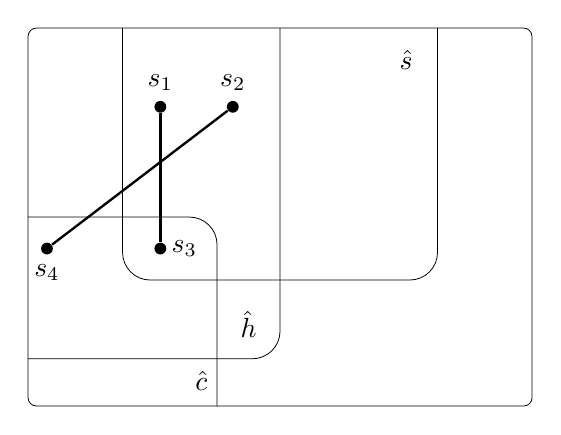
\begin{tikzpicture}[scale=0.8, every node/.style={circle, fill=black, inner sep=0.5pt, minimum size=1.5mm}]
		% \draw[help lines] (0,0) grid (8,6);
		\draw[rounded corners=3pt, line width=0.1mm] (0,0) rectangle (8,6); \draw[rounded
			corners=10pt, line width=0.1mm] (1.5, 6) -- (1.5,2) -- (6.5,2) -- (6.5,6); \draw[rounded
			corners=10pt, line width=0.1mm] (4,6) -- (4,0.75) -- (0,0.75); \draw[rounded
			corners=10pt, line width=0.1mm] (0,3) -- (3,3) -- (3,0);

		\node[fill=none] (h) at (3.5, 1.3) [] {$\hat{h}$};
		\node[fill=none] (s) at (6, 5.5) [] {$\hat{s}$};
		\node[fill=none] (c) at (2.75, 0.4) [] {$\hat{c}$};
		\node (1) at (2.1,4.75) [label=above:{$s_{1}$}] {};
		\node (2) at (3.25,4.75) [label=above:{$s_{2}$}] {};
		\node (3) at (2.1,2.5) [label=right:{	$s_{3}$}] {};
		\node (4)	at (0.3,2.5) [label=below:{	$s_{4}$}] {};
		\draw[line width=0.3mm] (1) -- (3);
		\draw[line width=0.3mm] (2) -- (4);
	\end{tikzpicture}
	\caption{The \textit{en passant} argument for allowing non-injective interpretations}
	\label{figure:duplicate-states-example}
\end{figure}

The preferential interpretation in \Cref{figure:duplicate-states-example} is not a model of $s \twiddle c$, due to
the counter example of $s_{2}$, which is a minimal $s$ -state that does not satisfy $c$. Should the duplicate
states be merged into $s_{12}$, so that now $s_{3}\prec s_{12}$ and $s_{4}\prec s_{12}$, then $s \twiddle c$ would
be satisfied, since $s_{12}$ is no longer an $s$-minimal state.

\subsection{Preferential Entailment}
\label{subsection:preferential-entailment}

Equipped with definitions for the class of preferential relations and a representation theorem that relates these
to a corresponding semantics derived from preferential interpretations, it is appropriate to discuss the matter of
\textit{preferential entailment}. Consider the following definition.

\begin{definition}
	\label{definition:p-entailment} \index{preferential!entailment} \index{entailment!preferential}

	A defeasible knowledge base $\Delta$ \textit{preferentially entails} a defeasible conditional $\phi \in \Lang$ if
	and only if $\phi$ is satisfied by every preferential model of $\Delta$. In this case we write $\Delta \pentails
		\phi$. The set of all defeasible conditionals that can be preferentially entailed from $\Delta$ is denoted by
	$\Cn{p}(\Delta)$ and is called the \textit{preferential closure} of $\Delta$.
\end{definition}

When we speak of the \textit{closure} of a set of preferential statements $\Delta$, described by the closure
operator $\Cn{p}(\Delta)$, it is reasonable to question whether what is really meant is a closure operator in the
sense of \Cref{definition:closure-operator}, or something else. Afterall, one property of closure operators is
that they are monotone, and so if we really do have a closure operator then $\Delta \subseteq \Delta'$ implies
that $\Cn{p}(\Delta) \subseteq \Cn{p}(\Delta')$. In other words, preferential entailment describes a monotone
relation. We begin by describing the closure system corresponding to $\Cn{p}$.

\begin{proposition}
	\label{proposition:entailemnt-relations-intersection}

	Let $\Delta$ be a defeasible knowledge base over $\Lang$, $\phi \twiddle \psi$ a defeasible statement in the same
	language, and $\mathfrak{W}$ be the set of all preferential relations induced by models of $\Delta$. Then, $\phi
		\twiddle \psi \in \Cn{p}(\Delta)$ if and only if $\phi \twiddle \psi \in \bigcap \mathfrak{W}$.
\end{proposition}

We abuse notation here, and use $\twiddle$ to mean the object-level connective, as well as to denote a
preferential consequence relation. It does not cause any issue, as the connective $\phi \twiddle \psi$ is
satisfied by a preferential model $\pin$ if and only if it is in the preferential relation $\twiddle_\pin$ induced
by $\pin$. The proposition states that the preferential consequence operator applied to $\Delta$ amounts to the
intersection of of the preferential consequence relations induced by the models of $\Delta$. The next proposition
confirms what might already be suspected: that preferential consequence relations are closed under arbitrary
intersections.

\begin{proposition}
	\label{proposition:intersection-preferential-relations}

	If $\mathfrak{W}$ is a set of preferential relations, then the intersection $\bigcap \mathfrak{W}$ is itself a
	preferential relation.
\end{proposition}

\begin{proof}
	\label{proof:intersection-preferential-relations}

	Let $\mathfrak{W}$ be a set of preferential relations and suppose the intersection, $\pin$, were not preferential.
	Then $\pin$ is not closed under application of \Crefrange{postulate:ref}{postulate:cm}. This means that there is
	some $\pin' \in \mathfrak{W}$ that is also not closed in the same way. Then $\pin'$ is not a preferential relation
	either, which is a contradiction.
\end{proof}

Indeed, the preferential consequence operator is a closure operator in the strict sense, and preferential
entailment is monotonic. The entailment relation can further be characterised by a single smallest preferential
consequence relation which, by \Cref{theorem:completeness-preferential}, \lucas{has a canonical model}.

\begin{theorem}
	\label{theorem:preferential-entailment-monotonic}

	Let $\Delta$ be a set of defeasible statements in $\Lang$, and $\Cn{p}(\Delta)$ its preferential closure. Then
	$\Cn{p}(\Delta)$ grows monotonically with $\Delta$.
\end{theorem}

\begin{proof}
	\label{proof:preferential-entailment-monotonic}

	Suppose that $\phi \twiddle \psi \in \Cn{p}(\Delta)$ and $\phi \twiddle \psi \not \in \Cn{p}(\Delta')$ with
	$\Delta \subseteq \Delta'$. For every model $\pin$ of $\Delta$ we have $\phi \twiddle_\pin \psi$ (this follows
	from \Cref{proposition:entailemnt-relations-intersection}), but also there exists a model $\mathcal{V}$ of
	$\Delta'$ such that $\phi \ntwiddle_\mathcal{V} \psi$. Since $\Delta \subseteq \Delta'$ we have that any model of
	$\Delta'$ is also a model of $\Delta$, then $\mathcal{V}$ is a model of $\Delta$ and so $\phi \twiddle \psi \not
		\in \Cn{p}(\Delta)$, which is a contradiction.
\end{proof}

There is room for some (justified) confusion here. After all, we have carefully avoided satisfying otherwise
useful properties because they imply monotonicity, only to end up with precisely that. To clarify this, we
recognise that a system can display non-monotonic behaviour in different areas. Indeed the entailment relation of
system P---which reasons on the metalevel---is monotonic, while the object level expresses non-monotonic
behaviour, facilitating the expression of statements like \textit{Normally Humans experience chronological-time},
\textit{Billy Pilgrim is a Human}, \textit{Billy Pilgrim experiences non-chronological time}. There are arguments,
in fact we make one in \Cref{section:preferential-contexts}, which suggest that object level non-monotonicity is
sufficient.

We now collect some further results which---apart from being interesting in their own right---will be useful in
the second part of this work.

\begin{corollary}
	\label{corollary:preferential-entailment-postulates}

	$\Delta \pentails \phi \twiddle \psi$ if and only if there is a proof from $\Delta$ to $\phi \twiddle \psi$ derived by
	application of \Crefrange{postulate:ref}{postulate:cm}.
\end{corollary}

It may have been presumed that, due to the resemblance of the postulates to Hilbert-style inference rules,
\Cref{corollary:preferential-entailment-postulates} would hold in quite a trivial sense. While this presumption
would be technically correct, we should proceed with caution. In a moment a system very close to preferential
reasoning will be presented, characterised by an almost identical set of postulates, for which the corresponding
version of this corollary fails. To grasp why it holds for preferential entailment, consider the following proof
\cite{kraus1990nonmonotonic}.

\begin{proof}
	\label{proof:preferential-entailment-postulates}

	We begin with the \textit{if} direction. For contraposition, assume that there is no proof from $\Delta$ to $\phi
		\twiddle \psi$ using the postulates. That is, if $\Delta$ were closed under application of the postulates, call
	this $\Delta^P$, then $\phi \twiddle \psi \not \in \Delta^P$. Need to finish this wording, basically show that all
	models of $\Delta$ have consequence relations that are preferential, and so $\Delta^P \subseteq \pin$ for any
	model.
\end{proof}

\subsection{Rational Consequence Relations}
\label{subsection:rational-consequence-relations}

System P provides a characterisation, in the form of its postulates, of a particular style of non-monotonic
reasoning. There are other kinds of reasoning, not valid in system P, for which there are good reasons think of as
reasonable properties of non-monotonic reasoning \cite{kraus1990nonmonotonic,lehmann1992what}.

\textit{Negation Rationality} suggests that our defeasible inferences should withstand piercing the veil of
ignorance. Suppose Alice is a university student, if she holds the belief that \textit{Normally, she will pass her
	exams}, then it would not be reasonable for her to simultaneously think \textit{Normally, if she studies, she will
	not pass her exams} and also \textit{Normally, if she does not study, she will not pass her exams}.
%
\begin{align}
	\inferLeft{Negation Rationality}{\phi \land \psi \ntwiddle \gamma, \quad \phi \land \neg \psi \ntwiddle \gamma}{\phi \ntwiddle \gamma}
\end{align}
%
While the example is possibly subject to the objection that a reasonable measure of whether one studied or not is
usually some degree of truth, rather than a binary, the point stands. Either Alice was sufficiently prepared or
she was not. If, in either case, she would not pass her exams, then it is difficult to comprehend how it might be
normal for her to pass her exams.

The \textit{Disjunctive Rationality} says that a plausible inference made from a disjunction should be plausible
from at least one of the disjuncts.
%
\begin{align}
	\inferLeft{Disjunctive Rationality}{\phi \ntwiddle \gamma, \quad \psi \ntwiddle \gamma}{\phi \lor \psi \ntwiddle \gamma}
\end{align}
%
\textit{Rational monotony} is a much stronger form of restricted monotony than cautious monotony. Where cautious
monotony holds the position that one should only reason monotonically with the addition of new information that
was already expected given our beliefs, rational monotony permits reasoning monotonically in the face of new
information that was merely \textit{consistent} with existing beliefs. Newly learned information may be considered
suprising when the initial epistemic position expects the opposite (\textit{[sic] negation}) to hold. Rational
monotony then corresponds to remaining in the monotonic realm, unless we truly are suprised by what is learned.
%
\begin{align}
	\inferLeft{Rational Monotony}{\phi \twiddle \psi, \quad \phi \ntwiddle \neg \gamma}{\phi \land \gamma \twiddle \psi}
\end{align}

At a university, it might be normal for students to graduate. At the same time, it would be too great a
requirement to suggest that it is normal for students to be exceptionally clever. It seems completely appropriate
to maintain our belief that it is normal for students, who are not exceptionally clever, to graduate.

%TODO Second reference is not Stalnaker
Stalnaker \cite{Stalnaker1994,sep-logic-nonmonotonic-Stanford}, and separately Ginsberg
\shortcite{GinsberCounterfactuals}, provide an argument against accepting rational monotony. The objection is that
rational monotony commits us to make inferences when the more reasonable position is to remain undecided.
Paraphrasing, we are asked to consider three composers: \textit{Verdi}, who is believed to be Italian, as well as
\textit{Satie} and \textit{Bizet}, who are believed to be French. If it were learned that Verdi and Bizet were
compatriots, then it seems reasonable that the conclusion that either of them are French or Italian is
indeterminate. What is reasonable, however, is to maintain the belief that Satie is French.\footnote{We will use
	some syntax from predicate logic, this is merely an aid to make Stalnaker's example clearer.}
%
\begin{align}
	\texttt{Compatriots(Bizet, Verdi)}\twiddle \texttt{French(Satie)}
\end{align}

The argument proceeds by considering that Verdi and Satie may too be compatriots. Since Verdi's nationality is now
unknown, we are no longer equipped to reject the plausibility of the new compatriotship, and so
%
\begin{align}
	\texttt{Compatriots(Bizet, Verdi)}\ntwiddle \neg \texttt{Compatriots(Verdi,Satie)}
\end{align}
%
The two conditions of rational monotony have been met, and so the following inference should continue to hold
%
\begin{align}
	\texttt{Compatriots(Bizet, Verdi)}\land \texttt{Compatriots(Verdi,Satie)}\twiddle \texttt{French(Satie)}
\end{align}

The issue, as Stalnaker sees it, is that rational monotony forces the inference Satie is still French, and by
their compatriotship, so are Bizet and Verdi. The ``correct'' thing to do in this scenario, as Stalnaker sees it,
would be to remain uncertain about which nationality they all share. However, the result that Stalnaker objects to
is dependent his particular construction of this problem, rather than being an intrinsic defect of rational
monotony. The second condition for rational monotony, that $\phi \ntwiddle \neg \gamma$, makes no requirement
about the syntactic structure of $\gamma$ outside of it being a formula in the language. In the example, Stalnaker
could just as easily have written
%
\begin{align}
	\texttt{Compatriots(Bizet,Verdi)}\ntwiddle \neg (\neg \texttt{Compatriots(Verdi,Satie))}
\end{align}
%
meaning that it is not expected that Verdi and Satie are compatriots, to which we can apply an instance of
rational monotony, from which we are not forced to believe that all three composers are French.
%
\begin{align}
	\texttt{Compatriots(Bizet, Verdi)}\land \neg(\texttt{Compatriots(Verdi,Satie))}\twiddle \texttt{French(Satie)}
\end{align}

There is another objection to rational monotony, which will be considered later on. For now, we accept it as a
valid property of non-monotonic reasoning, and thus introduce \textit{rational relations}.
%TODO argument against total preorders as representations of preference

\begin{definition}
	\label{definition:rational-relation} \index{rational!consequence relation}

	The consequence relation $\twiddle$ is a \emph{rational consequence relation} if and only if it satisfies the
	properties of \emph{Reflexivity}, \emph{Left Logical Equivalence}, \emph{Right Weakening}, \emph{And}, \emph{Or},
	\emph{Cautious Monotony}, and \emph{Rational Monotony}.
\end{definition}
%
Quite evidently, rational consequence relations are a particular kind of preferential consequence relation.

\subsubsection{Ranked Interpretations}
\label{subsubsection:ranked-interpretations}

From the knowledge that rational relations are a particular kind of preferential relation, it seems a reasonable
jump to think that the semantics we give to rational relations may be a particular kind of preferential
interpretation. Before discussing this jump, a useful exercise is to recognise how a preferential interpretation
may fail to be rational.

Consider the two preferential interpretations shown in \Cref{figure:two-preferential-models}. While they both
model the scenario that was discussed in the example near the end of the last subsection, the first does not
satisfy rational monotony.

\begin{example}
	\label{example:university}

	Suppose that neither Alice nor Bob are clever students. In spite of this, Alice is considered, by the preference
	relation, to be a normal student, alongside Charlie. This situation is modelled in each of the preferential
	interpretations below.

	\begin{figure}[H]
		\centering
		\begin{minipage}{0.49\textwidth}
			\centering
			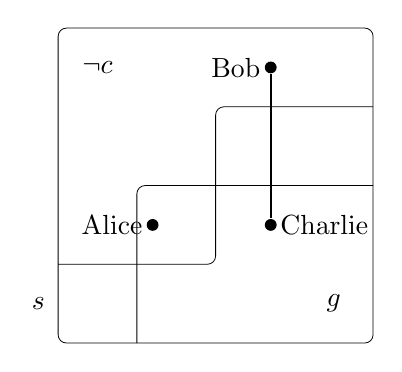
\begin{tikzpicture}[every node/.style={circle, fill=black, inner sep=0.5pt, minimum size=1.5mm}]

				\draw[rounded corners=3pt, line width=0.1mm] (0,0) rectangle (4,4);
				\draw[rounded corners=3pt, line width=0.1mm] (0,1) -- (2,1) -- (2,3) -- (4,3);
				\draw[rounded
					corners=3pt, line width=0.1mm] (1,0) -- (1,2) -- (4,2);

				\node[fill=none] (clever) at (0.5,3.5) [] {$\neg c$};
				\node[fill=none] (graduated) at (3.5,0.5) [] {$g$};
				\node[fill=none] (student) at (-0.25,0.5) [] {$s$};

				\node (bob) at (2.7,3.5) [label=left:{Bob}] {};
				\node (charlie) at (2.7,1.5) [label=right:{Charlie}] {};
				\draw[line width=0.3mm] (bob) -- (charlie);
				\node (alice) at (1.2,1.5) [label=left:{Alice}] {};
			\end{tikzpicture}

			\subcaption{Non-modular preference relation}

			\label{subfigure:not-rational}
		\end{minipage}
		\begin{minipage}{0.49\textwidth}
			\centering
			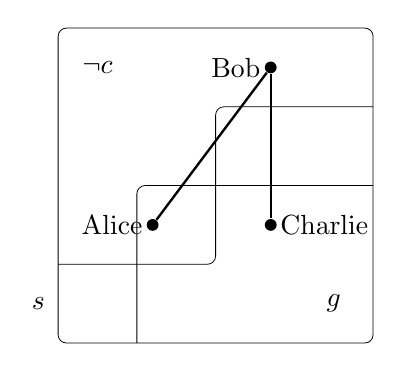
\begin{tikzpicture}[every node/.style={circle, fill=black, inner sep=0.5pt, minimum size=1.5mm}]

				\draw[rounded corners=3pt, line width=0.1mm] (0,0) rectangle (4,4);
				\draw[rounded corners=3pt, line width=0.1mm] (0,1) -- (2,1) -- (2,3) -- (4,3);
				\draw[rounded corners=3pt, line width=0.1mm] (1,0) -- (1,2) -- (4,2);

				\node[fill=none] (clever) at (0.5,3.5) [] {$\neg c$};
				\node[fill=none] (graduated) at (3.5,0.5) [] {$g$};
				\node[fill=none] (student) at (-0.25,0.5) [] {$s$};
				\node (bob) at (2.7,3.5) [label=left:{Bob}] {};
				\node (charlie) at (2.7,1.5) [label=right:{Charlie}] {};
				\draw[line width=0.3mm] (bob) -- (charlie);
				\node (alice) at (1.2,1.5) [label=left:{Alice}] {};
				\draw[line width=0.3mm] (bob) -- (alice);

			\end{tikzpicture}

			\subcaption{Modular preference relation} \label{subfigure:rational}
		\end{minipage}

		\caption{ Two preferential models of the above scenario} \label{figure:two-preferential-models}
	\end{figure}

	We may verify that both are models of $\texttt{student}\twiddle \texttt{graduate}$, and neither are models of
	$\texttt{student}\twiddle \texttt{clever}$. By rational monotony, we should expect that $\texttt{student}\land
		\neg \texttt{clever}\twiddle \texttt{graduate}$ be satisfied, which is not the case in
	\Cref{subfigure:not-rational}.
\end{example}

Fortunately, the reason behind \Cref{subfigure:not-rational}'s failure to satisfy rational monotony is easy to
identify. Bob, who is not considered when referring to the set of normal students, emerges as one of normal
students who are also not clever. This seems acceptable in isolation, but should not be possible due to Alice, who
is both a normal student and a normal, non-clever student. Her status as a normal student should position her as
more preferred to Bob, who is not a normal student. This preference extends when considering non-clever students,
and so Bob should not be considered a typical instance of this class.

In order to ensure rational monotony, it is required that the preference relation commit to Alice being preferred
to Bob; more generally, all normal students should be explicitly preferred to non-normal students. This
requirement is generalised as the property of \textit{modularity}:

\begin{definition}
	\label{definition:modular-order} \index{partial order! modular}

	A (strict) partial order $\prec$ on the set $X$ is \emph{modular} if and only if for any incomparable $x,y \in X$
	when $z \prec x$ then also $z \prec y$.
\end{definition}

One perspective on modular orders is that the incomparability relation between elements in such orders is required
to be transitive. Referring to \Cref{subfigure:not-rational}, observe that \textit{Bob} is incomparable to
\textit{Alice}, who is incomparable to \textit{Charlie}. If the order were modular, then \textit{Bob} should be
incomparable to \textit{Charlie}, which is obviously not the case. \textit{Ranked interpretations} are then
specialisations on preferential interpretations, defined below. The motivation for calling them \textit{ranked}
will be made clear in a moment.

\begin{definition}
	\label{definition:ranked-interpretation} \index{interpretation!ranked}

	A \emph{ranked interpretation} is a preferential interpretation $\Pin$ where the preference relation $\prec$ is
	\emph{modular}.
\end{definition}

Another, more intuitive understanding of modularity is that it partitions the carrier set into equivalence classes
such that all members of one equivalence class are incomparable to one another, but comparable to every other
element \cite{GinsberCounterfactuals}. Consider two states $s_1$ and $s_2$ in distinct equivalence classes, $C_1$
and $C_2$, respectively. Then suppose that $s_1$ is preferred to $s_2$, and so $s_1 \prec s_2$. By modularity, it
follows that $s_1$ is then preferred to every member of $C_2$, and moreover that every member of $C_1$ is
preferred to every member of $C_1$. In light of this fact, a simpler representation would be to consider a
preference ordering on quotient set of these equivalence classes, rather than the states themselves. One state is
preferred to another if it is a member of a more preferred equivalence class. This notion is made formal with the
following lemma, where preference is conveyed through the introduction of \textit{ranks}.

\begin{lemma}
	\label{lemma:modular-ranking-function}

	If $\prec$ is a modular, strict partial order on $X$ then there is a \emph{ranking function} $\mathsf{R} \colon X
		\to \Omega$, with $\Omega$ being a totally ordered set for which the strict order is denoted $<$, such that if $x
		\prec y$ then $\mathsf{R} (x) < \mathsf{R} (y)$ for any $x,y \in X$.
\end{lemma}

One pleasing consequence of this new approach to preference orders is that \Cref{lemma:states-preferential} is no
longer relevant, as the en passant style argument is avoided by the total order between ranks. As a result, the
ranking function need not consider states and may take the set of valuations as its domain. Ranked interpretations
are then redefined accordingly.

\begin{definition}
	\label{definition:ranked-interpretation-real}

	A \emph{ranked interpretation} is a function $\mathsf{R} \colon \Val \to \mathbb{N}$ that maps valuations to their
	\emph{rank}, given by a natural number.
\end{definition}

Another consequence is that ranked interpretations admit a new representation. Instead of Hasse diagrams, they may
be represented as stratified members of the equivalnce relation. As depicted in
\Cref{figure:ranked-interpretation-representation}, where each strata, or \textit{rank}, is associated with a
natural number.
%
\begin{figure}[H]
	\centering
	\captionsetup{width=0.3\textwidth}
	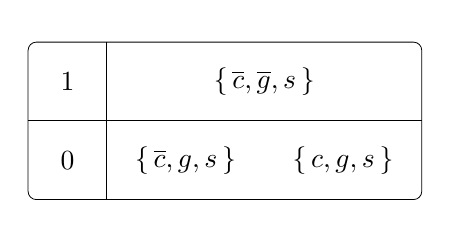
\begin{tikzpicture}[every node/.style={circle, fill=black, inner sep=0.5pt, minimum size=1.5mm}]
		\draw[rounded corners=3pt, line width=0.1mm] (-1,2) rectangle (4,0);
		\draw[rounded corners=3pt, line width=0.1mm] (-1,1) -- (4,1);
		\node[fill=none] (0) at (-0.5,0.5) [] {$0$};
		\node[fill=none] (1) at (-0.5,1.5) [] {$1$};
		\draw (0,0) -- (0,2);
		\node[fill=none] (alice) at (1,0.5) [] {$\{\,\overline{c},g,s\,\}$};
		\node[fill=none] (charlie) at (3,0.5) [] {$\{\,c,g,s\,\}$};
		\node[fill=none] (bob) at (2,1.5) [] {$\{\,\overline{c},\overline{g},s\,\}$};
	\end{tikzpicture}
	\caption{\Cref{subfigure:rational} represented as a ranked interpretation}
	\label{figure:ranked-interpretation-representation}
\end{figure}
%
If $\mathsf{R} $ is a ranking function under consideration, then $\mathsf{R} (v)$ denotes the rank of the
valuation $v$; and so, $\mathsf{R}(\{c,g,s\}) = 0$ in the above interpretation. Notice that the ranking funcion
that gives rise to \Cref{figure:ranked-interpretation-representation} does not appear to be defined for the
complete set of valuations. For instance, the valuation $\{\,\overline{c},\overline{g},\overline{s}\,\}$ does not
have a rank. While this is permissible, it may perhaps lead to questioning of \textit{why} certain valuations are
not considered. The most reasonable justification is that the excluded valuations, or possible worlds, should not
be possible under any circumstance.

It may then be more natural to add additional rank, the \textit{infinite rank}, to the co-domain of the ranking
function. Valuations that are mapped to the infinite rank then correspond to these \textit{impossible worlds}. The
notion of impossible worlds is important when considering how to derive information from a knowledge base
consisting of defeasible as well as classical statements. Intuitively, any valuations that are not models of the
classical statements should be regarded as impossible, and assigned the infinite rank.

\begin{definition}
	\label{definition:ranked-model-satisfaction}

	A ranked interpretation $\mathsf{R}$ is a model of a conditional $\phi \twiddle \psi$ if and only if every
	valuation $v$

\end{definition}

Need to add:
\begin{enumerate}[nosep]
	\item definitino of satisfaction w.r.t. ranking functions
	\item soundness \& completeness results (borign)
\end{enumerate}

\subsection{Ranked Entailment}
\label{subsection:ranked-entailment}

Considering that ranked interpretations are a particular kind of preferential interpretation, it may be
interesting to discuss the analagous entailment relation. Given that ranked interpretations restrict the kind of
preference orders to to those which are also modular---in doing so, causing the induced consequence relations to
be rational---it seems plausible that the entailment relation defined with respect to ranked models is indeed a
rational consequence relation.

\begin{definition}
	\label{definition:ranked-entailment}
	\index{entailment!ranked}

	A defeasible knowledge base $\Delta$ \emph{rank entails} a conditional $\phi \in \Lang$ if and only if $\phi$ is
	satisfied by every ranked model of $\Delta$. In this case we write $\Delta \dentails_R \phi$. The set of all
	conditionals that are rank entailed by $\Delta$ is denoted $\Cn{R}(\Delta)$.
\end{definition}

It immediately follows from the discussion on the monotonicity of preferential entailment that rank entailment is
indeed another Tarskian operator, and so is also monotonic. Rank entailment considers all ranked models of the set
$\Delta$. By the representation theorem, this corresponds to taking the intersection of the rational consequence
relations associated with each ranked model. While each of these is indeed rational, it is not necessary that
their intersection be. The example given below illustrates one reason why this may be.

\begin{example}
	\label{example:rank-entailment-example}

	Consider the two ranked interpretations below, which are models of the singleton knowledge base $\Delta =
		\{\texttt{student} \twiddle \texttt{graduate}\}$.

	\begin{figure}[H]
		\centering
		\begin{minipage}{0.45\textwidth}
			\centering
			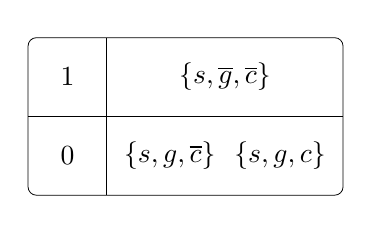
\begin{tikzpicture}[every node/.style={circle, fill=black, inner sep=0.5pt, minimum size=1.5mm}]
				\draw[rounded corners=3pt, line width=0.1mm] (0,2) rectangle (4,0);
				\draw[rounded corners=3pt, line width=0.1mm] (0,1) -- (4,1);
				\node[fill=none] (0) at (0.5,0.5) [] {$0$};
				\node[fill=none] (1) at (0.5,1.5) [] {$1$};
				\draw (1,0) -- (1,2);
				\node[fill=none] (alice) at (1.8,0.5) [] {$\{s,g,\overline{c}\}$};
				\node[fill=none] (bob) at (3.2,0.5) [] {$\{s,g,c\}$};
				\node[fill=none] (charlie) at (2.5,1.5) [] {$\{s,\overline{g},\overline{c}\}$};
			\end{tikzpicture}
			\subcaption{$\mathsf{R}_1$}
		\end{minipage}
		\begin{minipage}{0.45\textwidth}
			\centering
			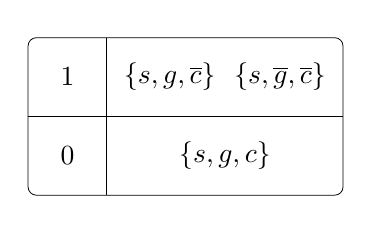
\begin{tikzpicture}[every node/.style={circle, fill=black, inner sep=0.5pt, minimum size=1.5mm}]
				\draw[rounded corners=3pt, line width=0.1mm] (0,2) rectangle (4,0);
				\draw[rounded corners=3pt, line width=0.1mm] (0,1) -- (4,1);
				\node[fill=none] (0) at (0.5,0.5) [] {$0$};
				\node[fill=none] (1) at (0.5,1.5) [] {$1$};
				\draw (1,0) -- (1,2);
				\node[fill=none] (alice) at (1.8,1.5) [] {$\{s,g,\overline{c}\}$};
				\node[fill=none] (bob) at (3.2,1.5) [] {$\{s,\overline{g},\overline{c}\}$};
				\node[fill=none] (charlie) at (2.5,0.5) [] {$\{s,g,c\}$};
			\end{tikzpicture}
			\subcaption{$\mathsf{R}_2$}
		\end{minipage}

		\caption{Two ranked models of $\Delta$}
	\end{figure}

	Let $\twiddle_1$ and $\twiddle_2$ be the consequence relations associated with each respective interpretation.
	Indeed, both are rational and contain the pair $(\texttt{student,graduate})$. Considering only $\twiddle_1$, it is
	easy to verify that
	%
	\begin{itemize}[nosep]
		\item $(\texttt{student,clever}) \not \in \,\twiddle_1$,
	\end{itemize}
	and by rationality (or inspection) that also,
	\begin{itemize}[nosep]
		\item $(\texttt{student} \land \neg \texttt{clever,graduate}) \in \, \twiddle_1$.
	\end{itemize}
	However, with respect to these two expressions, $\twiddle_2$ behaves in the opposite way:
	$(\texttt{student,clever})$ is included while $(\texttt{student}\land \neg \texttt{clever,graduate})$ is not. As a
	result, their intersection includes $(\texttt{student,graduate})$, does not include $(\texttt{student,clever})$.
	By rational monotony, $(\texttt{student}\land \neg \texttt{clever,graduate})$ should then also be included, but it
	is not. Accordingly, the relation is not rational.

\end{example}

Evidently rational consequence relations are not closed under intersections.

\section{Rational Closure}
\label{section:rational-closure}

Within the context of preferential models, there is another treatment of classical formulae which allows for the
discarding of \Cref{definition:state-satisfaction} and a single notion of what it means for a preferential
interpretation to be a model of a formula in $\Lang$. The idea is to translate the hard-constraints of classical
formulae to defeasible syntax.

\begin{lemma}
	\label{lemma:classical-to-defeasible}

	If $\phi$ is a classical formula in the language $\Lang$, then it can be expressed as the defeasible conditional
	$\neg \phi \twiddle \bot$. Then, any preferential interpretation $\pin$ is a model of $\phi$ if and only if it is
	a model of the defeasible conditional $\neg \phi \twiddle \bot$.
\end{lemma}

To explain the mechanics behind \Cref{lemma:classical-to-defeasible}, consider that a preferential interpretation
$\pin$ being a model of the conditional $\neg \phi \twiddle \bot$ is equivalent to the $\neg \phi$ -minimal states
being a subset of the states which satisfy $\bot$. Of course, $\bot$ represents logical falshood, and the set of
states which satisfy it is the emptyset. In turn, if $\pin$ is a model of $\neg \phi \twiddle \bot$, there can be
no states which satisfy $\neg \phi$, which is equivalent to the condition that all states satisfy $\phi$. If
$\phi$ is thought of as the proposition \say{All men are mortal}, then the defeasible counterpart reads as \say{If
	not all men are mortal, then it is normal to infer anything, including a contradiction}
\cite{kraus1990nonmonotonic,lehmann1992what}. We assume this treatment of classical formulae from this point
onwards, and consolidate the notation as $\pin \VDash \phi$ where $\phi \in \Lang$ is a defeasible conditional.
\textcolor{red}{maybe something about how without smoothness, we don't have CM}
%TODO This would not be the right place to add it. Rather it makes sense to add it in the section on preferential interpretations.
%TODO we have mentioned smoothness, so just reaffirm that it must hold

\begin{algo}{\textsc{BaseRank}}
	\label{algorithm:BaseRank}

	\Require A (finite) set $\Delta$ of defeasible conditionals in $\Lang$
	\Ensure A partition $(\Delta_{0}, \ldots, \Delta_{n}, \Delta_{\infty})$ of $\Delta$

	\State $i \coloneq 0$
	\State $\Gamma_{0}\coloneq \textsf{materialise}(\Delta)$

	\While{$\Gamma_{i}\not = \Gamma_{i-1}$}

	\State $\Gamma_{i+1}\coloneq \{\, \phi \rightarrow \psi \in \Gamma_{i}\colon \Gamma_{i}\vDash \neg \phi \,\}$
	\State $\Delta_{i}\coloneq \{\,\phi \twiddle \psi \colon (\phi \rightarrow \psi) \in \Gamma_{i}\setminus \Gamma_{i+1}\,\}$
	\State $i = i + 1$

	\EndWhile
	\State $\Delta_{\infty}\coloneq \Gamma_{i}$

	\If {$\Gamma_{i-1}= \emptyset$ }
	\State $n \coloneq i - 1$
	\Else
	\State $n \coloneq i - 2$
	\EndIf

	\State \Return $(\Delta_{0}, \ldots, \Delta_{n}, \Delta_{\infty})$
\end{algo}

\begin{algo}{\textsc{Rational Closure}}
	\label{algorithm:RationalClosureProp}

	\Require A set $\Delta$ of defeasible conditionals and a query $\phi \twiddle \psi$ from $\Lang$

	\Ensure \texttt{True} if $\Delta \dentails \phi \twiddle \psi$; \texttt{False}, otherwise.

	\State $(\Delta_{0}, \ldots, \Delta_{n}, \Delta_{\infty}) \coloneq \textsc{BaseRank}(\Delta )$

	\State $i \coloneq 0$

	\State $\Delta \coloneq \bigcup^{j<n}_{i=0}\Delta_{j}$

	\While {$\Delta_{\infty}\cup \Delta \vDash \neg \phi$ and $\Delta \not = \emptyset$ }

	\State $\Delta \coloneq \Delta \setminus \Delta_{i}$

	\State $i \coloneq i + 1$

	\EndWhile

	\State \Return $\Delta_{\infty}\cup \Delta \vDash \phi \twiddle \psi$
\end{algo}
